% Contenidos del capítulo
% Las secciones presentadas son orientativas y no representan
% necesariamente la organización que debe tener este capítulo.

\section{Requisitos}

En este capítulo se establecen los requisitos y las especificaciones de LocalMind-AI, un asistente de \gls{ia} orientado a la ejecución local. La definición parte del análisis del prototipo y de su arquitectura actual, pero se formula como un contrato verificable, por el que los requisitos expresan el comportamiento y las cualidades que deberá demostrar el sistema, no resultados que se consideren ya acreditados. Los objetivos cuantitativos se contrastarán posteriormente sobre los equipos de validación previstos.

La propuesta adopta un enfoque \gls{localfirst}, por el que la inferencia, los documentos y la memoria permanecen en el equipo de la persona usuaria de forma predeterminada \cite{kleppmann2019local}. Las integraciones que requieren acceder a servicios externos se consideran opcionales y solo podrán habilitarse tras una acción consciente y explícita. A partir de este principio se distinguen los requisitos funcionales, que describen las capacidades observables, y los requisitos no funcionales, que fijan restricciones y criterios de calidad.

\subsection{Requisitos funcionales}

Los requisitos funcionales definen las operaciones que LocalMind-AI deberá poner a disposición del usuario para las tareas de instalación, configuración y uso.

\begin{itemize}
    \item[\textbf{RF1.}] \textbf{Interacción conversacional y transparencia CoT.} El sistema deberá ofrecer un chat conversacional que muestre en tiempo real las respuestas incrementales del \gls{llm} y los pasos intermedios de razonamiento (\gls{cot}), indicando claramente cuándo el agente realiza reflexiones internas, consulta la memoria o invoca herramientas.
    \item[\textbf{RF2.}] \textbf{Gestión de conversaciones y tareas.} El sistema deberá permitir iniciar nuevas conversaciones, pausar o cancelar generaciones en curso, mantener el historial de mensajes por sesión, consultar y editar tareas asociadas y eliminar sesiones de forma segura.
    \item[\textbf{RF3.}] \textbf{Gestión y conmutación de modelos.} El sistema deberá permitir seleccionar y alternar dinámicamente el modelo de lenguaje en ejecución (\gls{ollama} o \gls{omlx}), validar la conectividad con el servidor de inferencia y adaptar la interfaz según el perfil de modelo activo.
    \item[\textbf{RF4.}] \textbf{Ingesta y procesamiento de documentos.} El sistema deberá permitir la carga de archivos en formatos \gls{pdf} y \gls{markdown}, su división en fragmentos semánticamente coherentes mediante \textit{recursive character text splitter} y su indexación vectorial en \gls{chromadb}.
    \item[\textbf{RF5.}] \textbf{Recuperación semántica (\gls{rag}).} El sistema deberá transformar las consultas del usuario en vectores de \gls{embeddings}, recuperar los $k$ fragmentos de código o documentación más relevantes de \gls{chromadb} e inyectarlos en el contexto del \gls{llm} para fundamentar la respuesta.
    \item[\textbf{RF6.}] \textbf{Configuración de parámetros \gls{rag}.} La interfaz deberá permitir ajustar el número de fragmentos a recuperar ($k$), el umbral de similitud semántica, el tamaño de fragmento (\textit{chunk size}) y el solapamiento (\textit{overlap}).
    \item[\textbf{RF7.}] \textbf{Persistencia de memoria semántica.} El sistema deberá integrar \gls{engram} para almacenar observaciones, aprendizajes y notas de la sesión, permitiendo la búsqueda por similitud sobre experiencias previas y su inyección transparente en el \gls{prompt} del agente.
    \item[\textbf{RF8.}] \textbf{Persistencia de sesiones y memoria.} El sistema deberá almacenar y recuperar el historial de las conversaciones mediante ficheros \gls{jsonl} y \gls{markdown}, y deberá permitir habilitar \gls{engram} como memoria persistente adicional. También deberá ofrecer mecanismos selectivos para eliminar estos datos.
    \item[\textbf{RF9.}] \textbf{Uso de herramientas.} El \gls{agenteia} deberá descubrir, habilitar e invocar herramientas proporcionadas mediante \gls{mcp}. El alcance funcional incluirá la generación de documentos \gls{pdf} y el almacenamiento de los artefactos resultantes en el equipo local. Las operaciones protegidas, como la ejecución de órdenes o la modificación de archivos, deberán requerir confirmación previa de la persona usuaria.
    \item[\textbf{RF10.}] \textbf{Seguimiento y recuperación.} La interfaz deberá comunicar los errores de conexión o ejecución, reintentar la conexión sin perder la sesión y mostrar un resumen comprensible de las etapas realizadas y de las herramientas utilizadas, sin exponer el contenido interno completo de la \gls{cot}.
\end{itemize}

\subsection{Requisitos no funcionales}

Los siguientes requisitos establecen criterios de calidad y umbrales de aceptación. Los valores temporales, de usabilidad y de consumo constituyen objetivos pendientes de validación en el apartado de pruebas de esta memoria.

\begin{itemize}
    \item[\textbf{RNF1.}] \textbf{Privacidad y funcionamiento local.} Los mensajes, documentos, índices, memorias e inferencias deberán procesarse localmente de forma predeterminada. Cualquier herramienta que transmita información fuera del equipo deberá permanecer deshabilitada hasta que la persona usuaria la active o autorice explícitamente.
    \item[\textbf{RNF2.}] \textbf{Latencia.} En las pruebas con el modelo de referencia, el percentil 90 del tiempo transcurrido hasta recibir el primer fragmento de una respuesta incremental deberá ser inferior o igual a 10 segundos. El cumplimiento se medirá por separado en el MSI Pulse GL66 y en el MacBook Air M4.
    \item[\textbf{RNF3.}] \textbf{Uso de recursos.} El servicio de \gls{nanobot} ejecutado en su contenedor tendrá un límite de 4~GiB de memoria. El consumo del contenedor \texttt{frontend} se evaluará de manera independiente y su imagen de ejecución no deberá conservar las dependencias utilizadas para construir el cliente. La selección del modelo deberá tener en cuenta la memoria principal y la memoria de vídeo disponibles, mientras que el consumo del motor de inferencia nativo se medirá por separado.
    \item[\textbf{RNF4.}] \textbf{Operación sin conexión.} Una vez instaladas las dependencias y descargados los modelos, el chat, la recuperación documental, la memoria y las herramientas locales deberán funcionar sin conexión a Internet. Las integraciones externas deberán indicar claramente su estado no disponible, sin impedir el uso de las funciones locales.
    \item[\textbf{RNF5.}] \textbf{Seguridad de red, privilegios y secretos.} Los servicios deberán enlazarse de forma predeterminada a la interfaz de red de bucle local. El contenedor de \gls{nanobot} deberá ejecutarse con un usuario sin privilegios, sin extender esta garantía a componentes que no se hayan validado. Una eventual exposición remota requerirá autenticación y cifrado mediante \gls{tls}; las credenciales no deberán almacenarse en el código fuente ni aparecer en respuestas o registros. Estas medidas se revisarán tomando como referencia las recomendaciones de \gls{owasp} \cite{OWASPTopTen}.
    \item[\textbf{RNF6.}] \textbf{Protección de acciones.} La ejecución de órdenes y la escritura, edición o eliminación de archivos deberán solicitar confirmación previa y limitarse al espacio de trabajo o a la política de aislamiento configurados.
    \item[\textbf{RNF7.}] \textbf{Fiabilidad de la comunicación.} Ante una interrupción recuperable, el cliente deberá restablecer la conexión en un máximo de 5 segundos, conservar la sesión activa y evitar la duplicación de solicitudes o resultados.
    \item[\textbf{RNF8.}] \textbf{Usabilidad.} La evaluación deberá alcanzar una puntuación \gls{sus} igual o superior a 68 y una tasa de éxito igual o superior al 80\,\% en las tareas de iniciar una conversación, cambiar el modelo y localizar un artefacto generado.
    \item[\textbf{RNF9.}] \textbf{Compatibilidad.} El cliente deberá funcionar en navegadores web modernos y los lanzadores deberán admitir \gls{macos}, \gls{linux} y \gls{windows}. \gls{omlx} se destinará a equipos Apple Silicon y \gls{ollama} constituirá la alternativa general.
    \item[\textbf{RNF10.}] \textbf{Reproducibilidad.} La instalación sobre un entorno limpio deberá poder completarse mediante el lanzador y la \gls{tui}, sin exigir la edición manual de los archivos de configuración generados. El cliente web deberá poder construirse y arrancarse mediante \gls{docker}, sin requerir \gls{nodejs}, \gls{pnpm} ni un directorio \texttt{node\_modules} como dependencias finales instaladas en el anfitrión.
    \item[\textbf{RNF11.}] \textbf{Mantenibilidad y extensibilidad.} Los módulos deberán estar documentados y seguir \gls{pep8} y los principios \gls{solid} \cite{PEP8Style,SOLIDPrinciplesCinco2025}. La incorporación de un nuevo proveedor de inferencia o servidor \gls{mcp} no deberá requerir modificaciones en el núcleo de la conversación.
    \item[\textbf{RNF12.}] \textbf{Persistencia.} El espacio de trabajo, las sesiones, la colección de \gls{chromadb}, la memoria de \gls{engram} y los artefactos generados por \gls{nanobot} deberán conservarse tras reiniciar o recrear los contenedores. Las operaciones de limpieza selectiva deberán afectar únicamente al almacén elegido.
    \item[\textbf{RNF13.}] \textbf{Observabilidad.} Los diagnósticos, indicadores de estado, comprobaciones de salud y registros deberán reflejar por separado la disponibilidad del cliente servido por \gls{nginx}, del agente, del motor de inferencia, de los servidores \gls{mcp} y de los almacenes persistentes, sin revelar datos sensibles.
    \item[\textbf{RNF14.}] \textbf{Trazabilidad y calidad.} Cada requisito funcional y no funcional deberá asociarse en la fase de validación con una prueba o evidencia reproducible. La clasificación de las características de calidad seguirá el modelo ISO/IEC~25010 \cite{ISOIEC25010}.
\end{itemize}

\section{Especificaciones}\label{sec:especificaciones-sistema}

A partir de los requisitos anteriores, LocalMind-AI se especifica como un sistema personal de asistencia local cuyo actor principal es una persona con conocimientos técnicos que instala, configura y utiliza el mismo entorno. No se establecen roles independientes de administración ni un modelo multiusuario. La solución se organiza en cuatro subsistemas, que corresponden a interacción, comunicación, aplicación y servicios locales. La Figura~\ref{fig:localmind-overview} resume su relación y diferencia mediante trazo discontinuo las integraciones externas, que son opcionales y requieren consentimiento.

\begin{figure}[htbp]
    \centering
    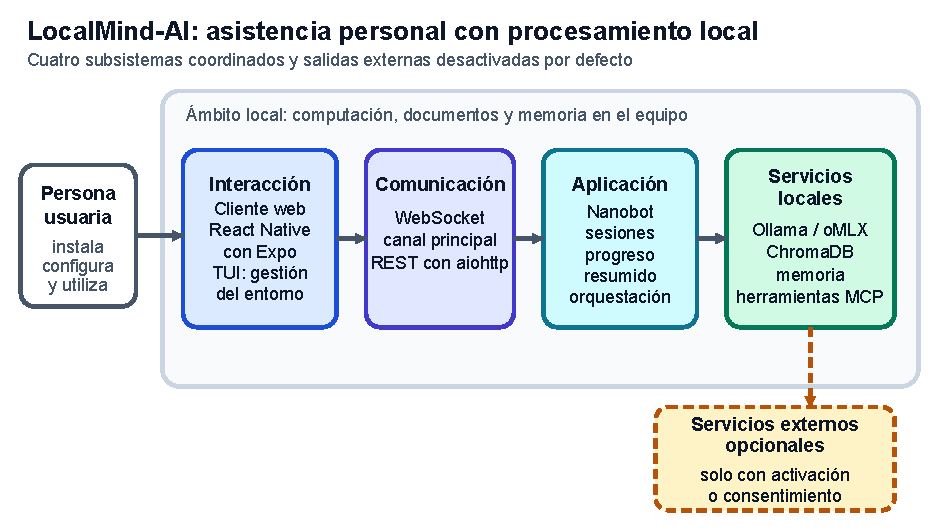
\includegraphics[width=0.95\textwidth]{figs/localmind-overview.pdf}
    \caption{Mapa conceptual de LocalMind-AI.}
    \label{fig:localmind-overview}
\end{figure}

El entorno de ejecución se distribuye entre el navegador, el equipo anfitrión y dos servicios gestionados mediante \gls{dockercompose}. Como representa la Figura~\ref{fig:localmind-runtime}, el servicio \texttt{frontend} contiene los activos estáticos exportados por \gls{expo} y los sirve mediante \gls{nginx} en el puerto 8081, mientras que el servicio \texttt{nanobot} aloja el agente, la pasarela \gls{websocket}, la \gls{api} \gls{rest} y las herramientas integradas. La imagen del agente se construye en varias etapas y su proceso se ejecuta con el usuario no privilegiado \texttt{nanobot} \cite{docker2026multistage}. Los servidores \gls{mcp}, incluido \gls{engram} cuando está habilitado, se inician dentro de ese contenedor como subprocesos configurados y no como servicios adicionales de Compose. \Gls{ollama} o \gls{omlx}, servidor basado en MLX, permanecen en el anfitrión para aprovechar la aceleración disponible y son accesibles desde el agente mediante \texttt{host.docker.internal} \cite{docker2024compose}.

\Gls{nginx} se limita a entregar la aplicación web y no actúa como proxy inverso de los canales del agente \cite{nginx2026}. Después de descargar los activos desde \texttt{http://localhost:8081}, el navegador establece directamente con \gls{nanobot} la conexión \gls{websocket} del puerto 8765 o las peticiones \gls{rest} del puerto 8900. Como parte del diseño previsto, los volúmenes deberán separar el espacio de trabajo, las sesiones, los resultados, la colección vectorial y la memoria, además de conservar los datos exigidos por el RNF12 tras reinicios o recreaciones. Este comportamiento y las comprobaciones de salud definidas por el RNF13 permanecen pendientes de validación.

\begin{figure}[htbp]
    \centering
    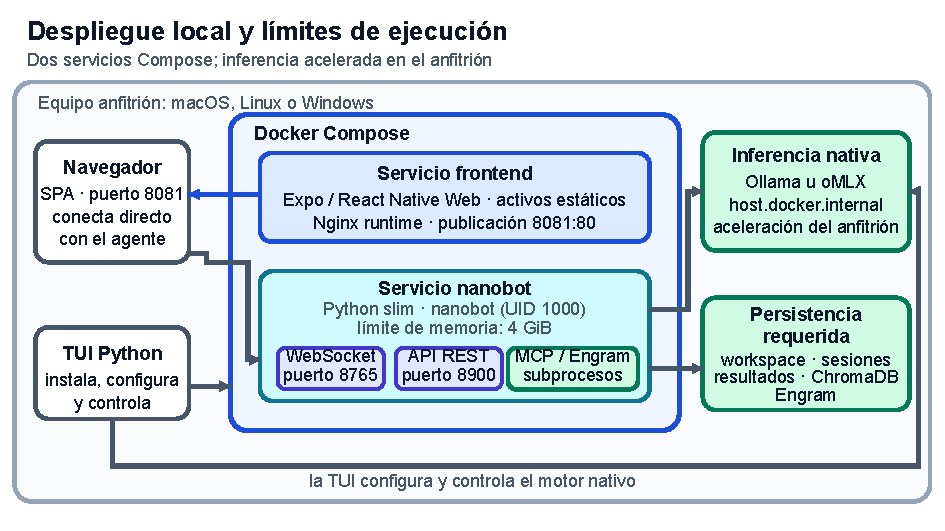
\includegraphics[width=0.95\textwidth]{figs/localmind-runtime.pdf}
    \caption{Entorno de ejecución local de LocalMind-AI.}
    \label{fig:localmind-runtime}
\end{figure}

La capa de interacción ofrece dos puntos de entrada complementarios, pero con responsabilidades distintas. El cliente desarrollado con \gls{reactnative} y \gls{expo}, exportado como aplicación web estática y servido por \gls{nginx}, proporciona la conversación en el navegador, la selección del modelo y la consulta de resultados \cite{meta2024reactnative,expo2024,nginx2026}. Una vez cargado, este cliente se conecta directamente con el servidor \gls{websocket} de \gls{nanobot} como canal principal para recibir eventos y fragmentos de respuesta, y dispone de una \gls{api} \gls{rest}, implementada con \gls{aiohttp} y compatible con el formato de conversación de OpenAI, como alternativa \cite{aiohttp2026,rfc6455}. Por separado, la \gls{tui}, implementada en \gls{python}, concentra la instalación, la configuración, el diagnóstico y el control operativo de \gls{dockercompose} y del motor nativo, por lo que no actúa como un cliente conversacional de esos dos canales. Esta separación se sintetiza en la Figura~\ref{fig:localmind-interaction}.

\begin{figure}[htbp]
    \centering
    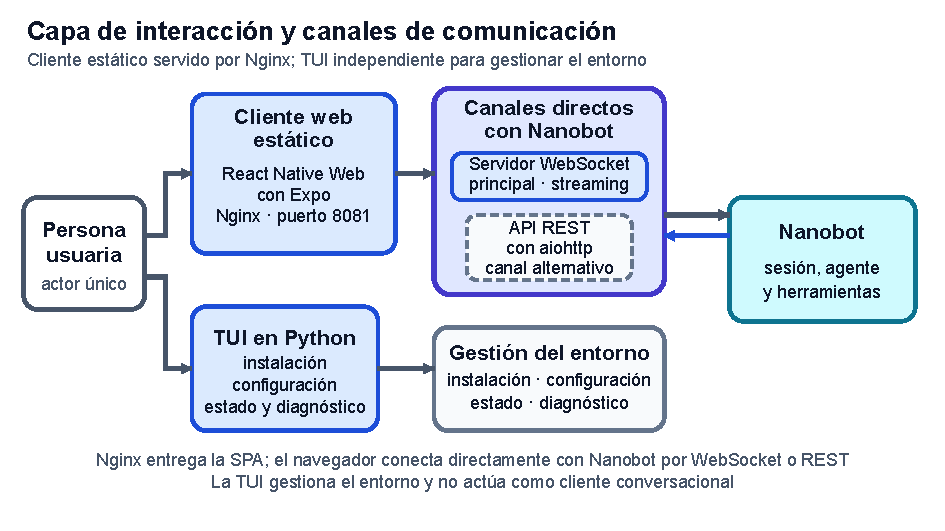
\includegraphics[width=0.95\textwidth]{figs/localmind-interaction.pdf}
    \caption{Mapa conceptual de la capa de interacción.}
    \label{fig:localmind-interaction}
\end{figure}

La capa de aplicación está constituida por \gls{nanobot}, que mantiene el contexto de la sesión, coordina las llamadas al modelo y selecciona las herramientas necesarias \cite{nanobot2026}. Según el flujo conceptual de la Figura~\ref{fig:localmind-agent}, cada petición se vincula primero con una sesión y, a continuación, el agente decide si puede responder mediante inferencia directa, si necesita recuperar documentación o si debe invocar una herramienta. Como comportamiento requerido, la interfaz deberá recibir estados resumidos y los nombres de las herramientas empleadas, pero no el razonamiento interno completo del modelo. Asimismo, los errores deberán convertirse en estados comprensibles y las acciones protegidas deberán introducir un punto de confirmación antes de continuar. El cumplimiento de este seguimiento visible y de la recuperación ante fallos queda pendiente de validación.

\begin{figure}[htbp]
    \centering
    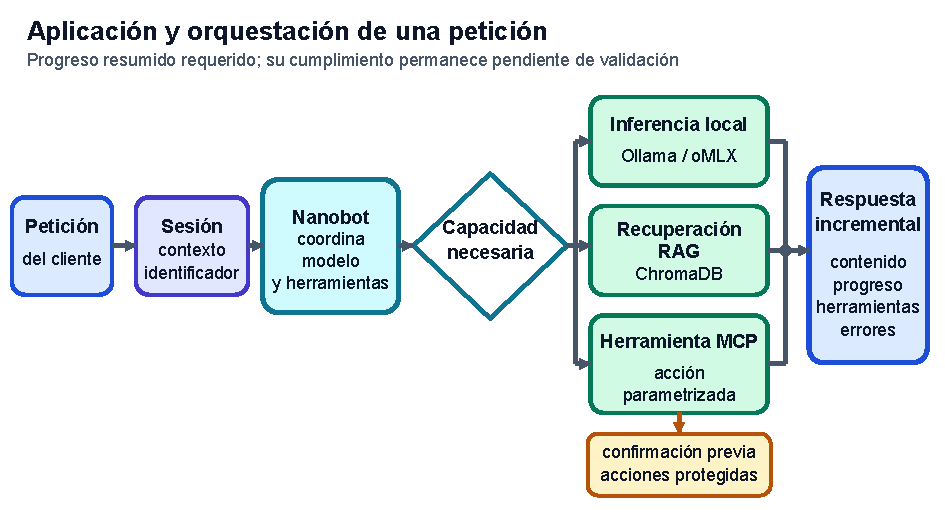
\includegraphics[width=0.95\textwidth]{figs/localmind-agent.pdf}
    \caption{Mapa conceptual de la capa de aplicación y orquestación.}
    \label{fig:localmind-agent}
\end{figure}

La capa de servicios, representada en la Figura~\ref{fig:localmind-services}, mantiene responsabilidades diferenciadas. \Gls{ollama} y \gls{omlx}, este último como servidor basado en \gls{mlx}, proporcionan inferencia local, \gls{chromadb} conserva los vectores empleados por \gls{rag}, los ficheros \gls{jsonl} y \gls{markdown} registran las sesiones, y \gls{engram} aporta, cuando se activa, una memoria semántica de mayor duración. Por su parte, \gls{mcp} normaliza el acceso del agente a herramientas locales o externas e incluye capacidades reales para generar documentos \gls{pdf} y guardar los artefactos correspondientes en el almacenamiento local \cite{ollama2024,omlx2026,chroma2026,anthropic2024mcp}. Estas piezas no son alternativas equivalentes, ya que cada una resuelve una responsabilidad distinta y puede evolucionar sin alterar el canal de interacción.

\begin{figure}[htbp]
    \centering
    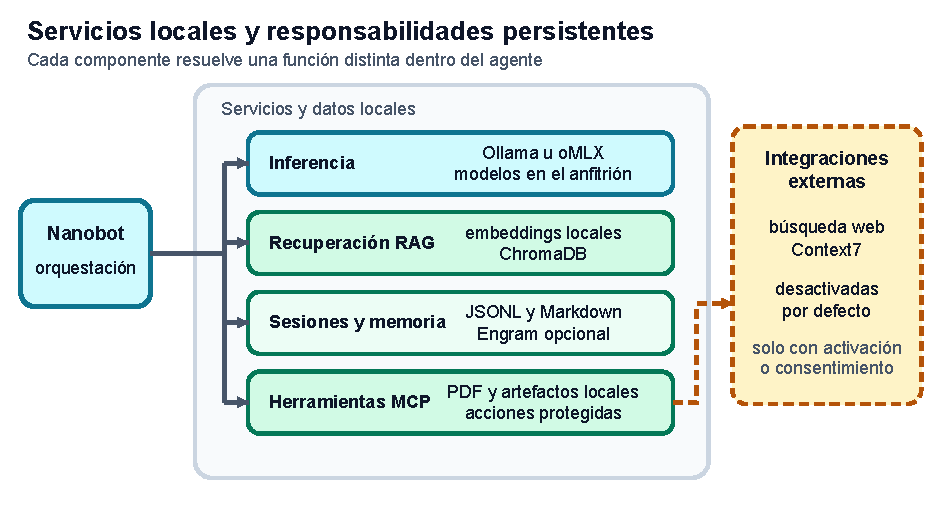
\includegraphics[width=0.95\textwidth]{figs/localmind-services.pdf}
    \caption{Mapa conceptual de los servicios locales.}
    \label{fig:localmind-services}
\end{figure}

La especificación excluye del alcance actual las cuentas de usuario, la administración remota y la infraestructura como servicio.

\FloatBarrier
\section{Costes}
% Costes temporales y económicos
En este apartado se presenta la planificación temporal del proyecto y se estima el coste económico asociado a su desarrollo. Para ello, se describe el ciclo de vida adoptado, se descompone el trabajo en actividades verificables y se valoran tanto la dedicación del autor como los medios materiales utilizados.

La elección de una metodología adecuada resulta necesaria para organizar el trabajo y controlar sus posibles desviaciones. Las \glspl{metagil} \cite{ilievaAnalysesAgileMethodology2004}, entre las que se encuentran \gls{scrum} y \gls{kanban}, favorecen ciclos breves, una adaptación continua y la interacción frecuente con las partes interesadas. Frente a ellas, los enfoques iterativos e incrementales estructuran el desarrollo en sucesivas revisiones de análisis, diseño, implementación y prueba, de forma que cada incremento se apoya en resultados previamente consolidados.

En LocalMind-AI se ha adoptado una \gls{iterativa} \cite{larmanIterativeIncrementalDevelopments2003}. Esta elección responde al carácter individual del proyecto y a la necesidad de validar de manera progresiva componentes con dependencias distintas, como el cliente web, el agente, la recuperación documental y los motores de inferencia. El enfoque conserva una planificación estructurada, pero permite revisar decisiones técnicas cuando una prueba de integración o una ejecución en otra plataforma revela una limitación no prevista.

El ciclo de vida se divide en seis fases principales. La fase de \textbf{documentación} comprende la revisión del estado del arte, la elaboración de prototipos y la redacción continuada de la memoria. La fase de \textbf{análisis} concreta los requisitos y las especificaciones. Durante el \textbf{diseño} se definen la arquitectura \gls{localfirst}, la interacción mediante el cliente web y la \gls{tui}, la comunicación, el agente, la recuperación documental y la inferencia local. La \textbf{implementación} materializa esos componentes e integra los dos servicios de \gls{dockercompose} con los motores que permanecen en el anfitrión. El \textbf{despliegue} prepara un entorno reproducible y comprueba la instalación en los dos equipos de validación. Por último, las \textbf{pruebas} reúnen la verificación funcional, de integración, rendimiento, recursos, usabilidad y seguridad.

La estimación de las actividades se ha realizado mediante la técnica \gls{pert} \cite{mazlumCPMPERTProject2015}. Esta técnica combina una duración optimista (\(O\)), una pesimista (\(P\)) y una duración más probable (\(M\)). La Ecuación~\ref{eq:tecnicaPERT} obtiene la duración esperada \(E\) mediante una media ponderada que concede mayor peso al escenario más probable.

% Ecuación técnica PERT.
\begin{equation}
    E = \frac{O + P + 4M}{6}
    \label{eq:tecnicaPERT}
\end{equation}

El desarrollo del \gls{tfm} se compagina con una jornada laboral ordinaria de ocho horas diarias en una empresa. Esas cuarenta horas semanales no forman parte del esfuerzo del proyecto y limitan la disponibilidad a los periodos indicados en la Tabla~\ref{tab:horarioTFM}. Se mantiene una dedicación de dos horas los jueves y viernes y de cuatro horas los sábados y domingos, lo que proporciona doce horas semanales.

% Tabla de horario de dedicación al TFM.
\begin{table}[h!tp]
    \centering
    \begin{adjustbox}{max width=\textwidth}
        \begin{tabular}{|c|c|c|c|c|c|c|c|}
            \hline
            Lunes & Martes & Miércoles & Jueves & Viernes & Sábado & Domingo & Total \\ \hline
            0 h   & 0 h    & 0 h       & 2 h    & 2 h     & 4 h    & 4 h     & 12 h  \\ \hline
        \end{tabular}
    \end{adjustbox}
    \caption{Horario semanal de dedicación al \gls{tfm}.}
    \label{tab:horarioTFM}
\end{table}

La Tabla~\ref{tab:estimacionTareas} recoge las veinticinco actividades previstas. La última columna expresa la duración esperada en semanas de doce horas; el total se calcula a partir de las horas sin redondear, por lo que no depende de la suma de los valores decimales mostrados en cada fila.

\sisetup{
    output-decimal-marker = {,},
    group-separator = {.}
}

\begin{table}[p]
    \centering
    \scriptsize
    \setlength{\tabcolsep}{2.5pt}
    \renewcommand{\arraystretch}{1.12}
    \begin{tabularx}{\textwidth}{
            |>{\raggedright\arraybackslash}p{2.2cm}
            |>{\raggedright\arraybackslash}X
            |S[table-format=2.0]
            |S[table-format=2.0]
            |S[table-format=2.0]
            |S[table-format=3.0]
            |S[table-format=2.2]|
        }
        \hline
        \textbf{Fase}                        & \textbf{Actividad}                                  & {\textbf{T. opt. (h)}} & {\textbf{T. pes. (h)}} & {\textbf{T. más probable (h)}} & {\textbf{Estim. (h)}}               & {\textbf{Semanas}} \\
        \hline
        \multirow{2}{=}{\centering Documentación}
                                             & Estado del arte y prototipos                        & 12                     & 24                     & 18                             & 18                                  & 1.50               \\
                                             & Redacción y revisión de la memoria                  & 18                     & 36                     & 27                             & 27                                  & 2.25               \\
        \hline
        \multirow{2}{=}{\centering Análisis}
                                             & Definición de requisitos                            & 8                      & 16                     & 12                             & 12                                  & 1.00               \\
                                             & Especificación del sistema                          & 10                     & 18                     & 14                             & 14                                  & 1.17               \\
        \hline
        \multirow{6}{=}{\centering Diseño}
                                             & Arquitectura \gls{localfirst} y despliegue          & 10                     & 22                     & 16                             & 16                                  & 1.33               \\
                                             & Interacción web y \gls{tui}                         & 6                      & 14                     & 10                             & 10                                  & 0.83               \\
                                             & Comunicación \gls{websocket}/\gls{rest}             & 6                      & 14                     & 10                             & 10                                  & 0.83               \\
                                             & Agente, \gls{mcp} y memoria                         & 8                      & 16                     & 12                             & 12                                  & 1.00               \\
                                             & \gls{rag}, \gls{chromadb} y \glspl{embeddings}      & 6                      & 14                     & 10                             & 10                                  & 0.83               \\
                                             & Inferencia local y multiplataforma                  & 10                     & 18                     & 14                             & 14                                  & 1.17               \\
        \hline
        \multirow{9}{=}{\centering Implementación}
                                             & \gls{tui} y lanzadores                              & 14                     & 30                     & 22                             & 22                                  & 1.83               \\
                                             & Cliente \gls{expo}/\gls{reactnative} Web            & 16                     & 36                     & 26                             & 26                                  & 2.17               \\
                                             & Exportación estática y \gls{nginx}                  & 8                      & 20                     & 14                             & 14                                  & 1.17               \\
                                             & Pasarela \gls{aiohttp} \gls{websocket}/\gls{rest}   & 16                     & 32                     & 24                             & 24                                  & 2.00               \\
                                             & \gls{rag}, \gls{chromadb} y \glspl{embeddings}      & 12                     & 28                     & 20                             & 20                                  & 1.67               \\
                                             & Sesiones, \gls{jsonl}/\gls{markdown} y \gls{engram} & 10                     & 22                     & 16                             & 16                                  & 1.33               \\
                                             & Herramientas \gls{mcp} y confirmaciones             & 10                     & 22                     & 16                             & 16                                  & 1.33               \\
                                             & Proveedores \gls{ollama}/\gls{omlx}                 & 8                      & 16                     & 12                             & 12                                  & 1.00               \\
                                             & Dockerfiles, Compose e integración                  & 6                      & 14                     & 10                             & 10                                  & 0.83               \\
        \hline
        \multirow{3}{=}{\centering Despliegue}
                                             & Entorno reproducible                                & 6                      & 14                     & 10                             & 10                                  & 0.83               \\
                                             & Validación MSI/\gls{windows}                        & 6                      & 14                     & 10                             & 10                                  & 0.83               \\
                                             & Validación MacBook/\gls{macos}                      & 6                      & 14                     & 10                             & 10                                  & 0.83               \\
        \hline
        \multirow{3}{=}{\centering Pruebas}
                                             & Pruebas funcionales e integración                   & 6                      & 14                     & 10                             & 10                                  & 0.83               \\
                                             & Rendimiento y recursos                              & 4                      & 10                     & 7                              & 7                                   & 0.58               \\
                                             & Usabilidad, seguridad y aceptación                  & 6                      & 14                     & 10                             & 10                                  & 0.83               \\
        \hline
        \multicolumn{2}{|l|}{\textbf{Total}} & \textbf{228}                                        & \textbf{492}           & \textbf{360}           & \textbf{360}                   & \multicolumn{1}{c|}{\textbf{30,00}}                      \\
        \hline
    \end{tabularx}
    \caption{Estimación de tareas del proyecto mediante la técnica PERT.}
    \label{tab:estimacionTareas}
\end{table}

La estimación esperada asciende a 360 horas, equivalentes a treinta semanas de dedicación. Para absorber incertidumbres se incorpora un margen del 10\,\%, es decir, 36 horas adicionales, con lo que el presupuesto temporal alcanza 396 horas. Entre el 7 de enero y el 28 de agosto de 2026, el patrón semanal definido proporciona 400 horas disponibles, sin descontar festivos ni vacaciones. La planificación conserva, por tanto, una holgura residual de cuatro horas.

La distribución temporal se representa mediante el \gls{gantt} de la Figura~\ref{fig:diagramaGantt}. La redacción de la memoria se mantiene en paralelo durante todo el proyecto, mientras que el estado del arte, el análisis, el diseño, la implementación, el despliegue y las pruebas avanzan de manera predominantemente secuencial. Los solapamientos de un día entre fases representan el reparto de las horas disponibles dentro de esa jornada y no dos jornadas completas de trabajo simultáneo. Se reserva, además, el periodo comprendido entre el 6 y el 23 de agosto para contingencias y correcciones, y los días 27 y 28 de agosto como holgura no comprometida antes de la entrega.

% Diagrama de Gantt del proyecto.
\begin{sidewaysfigure}[p]
    \centering
    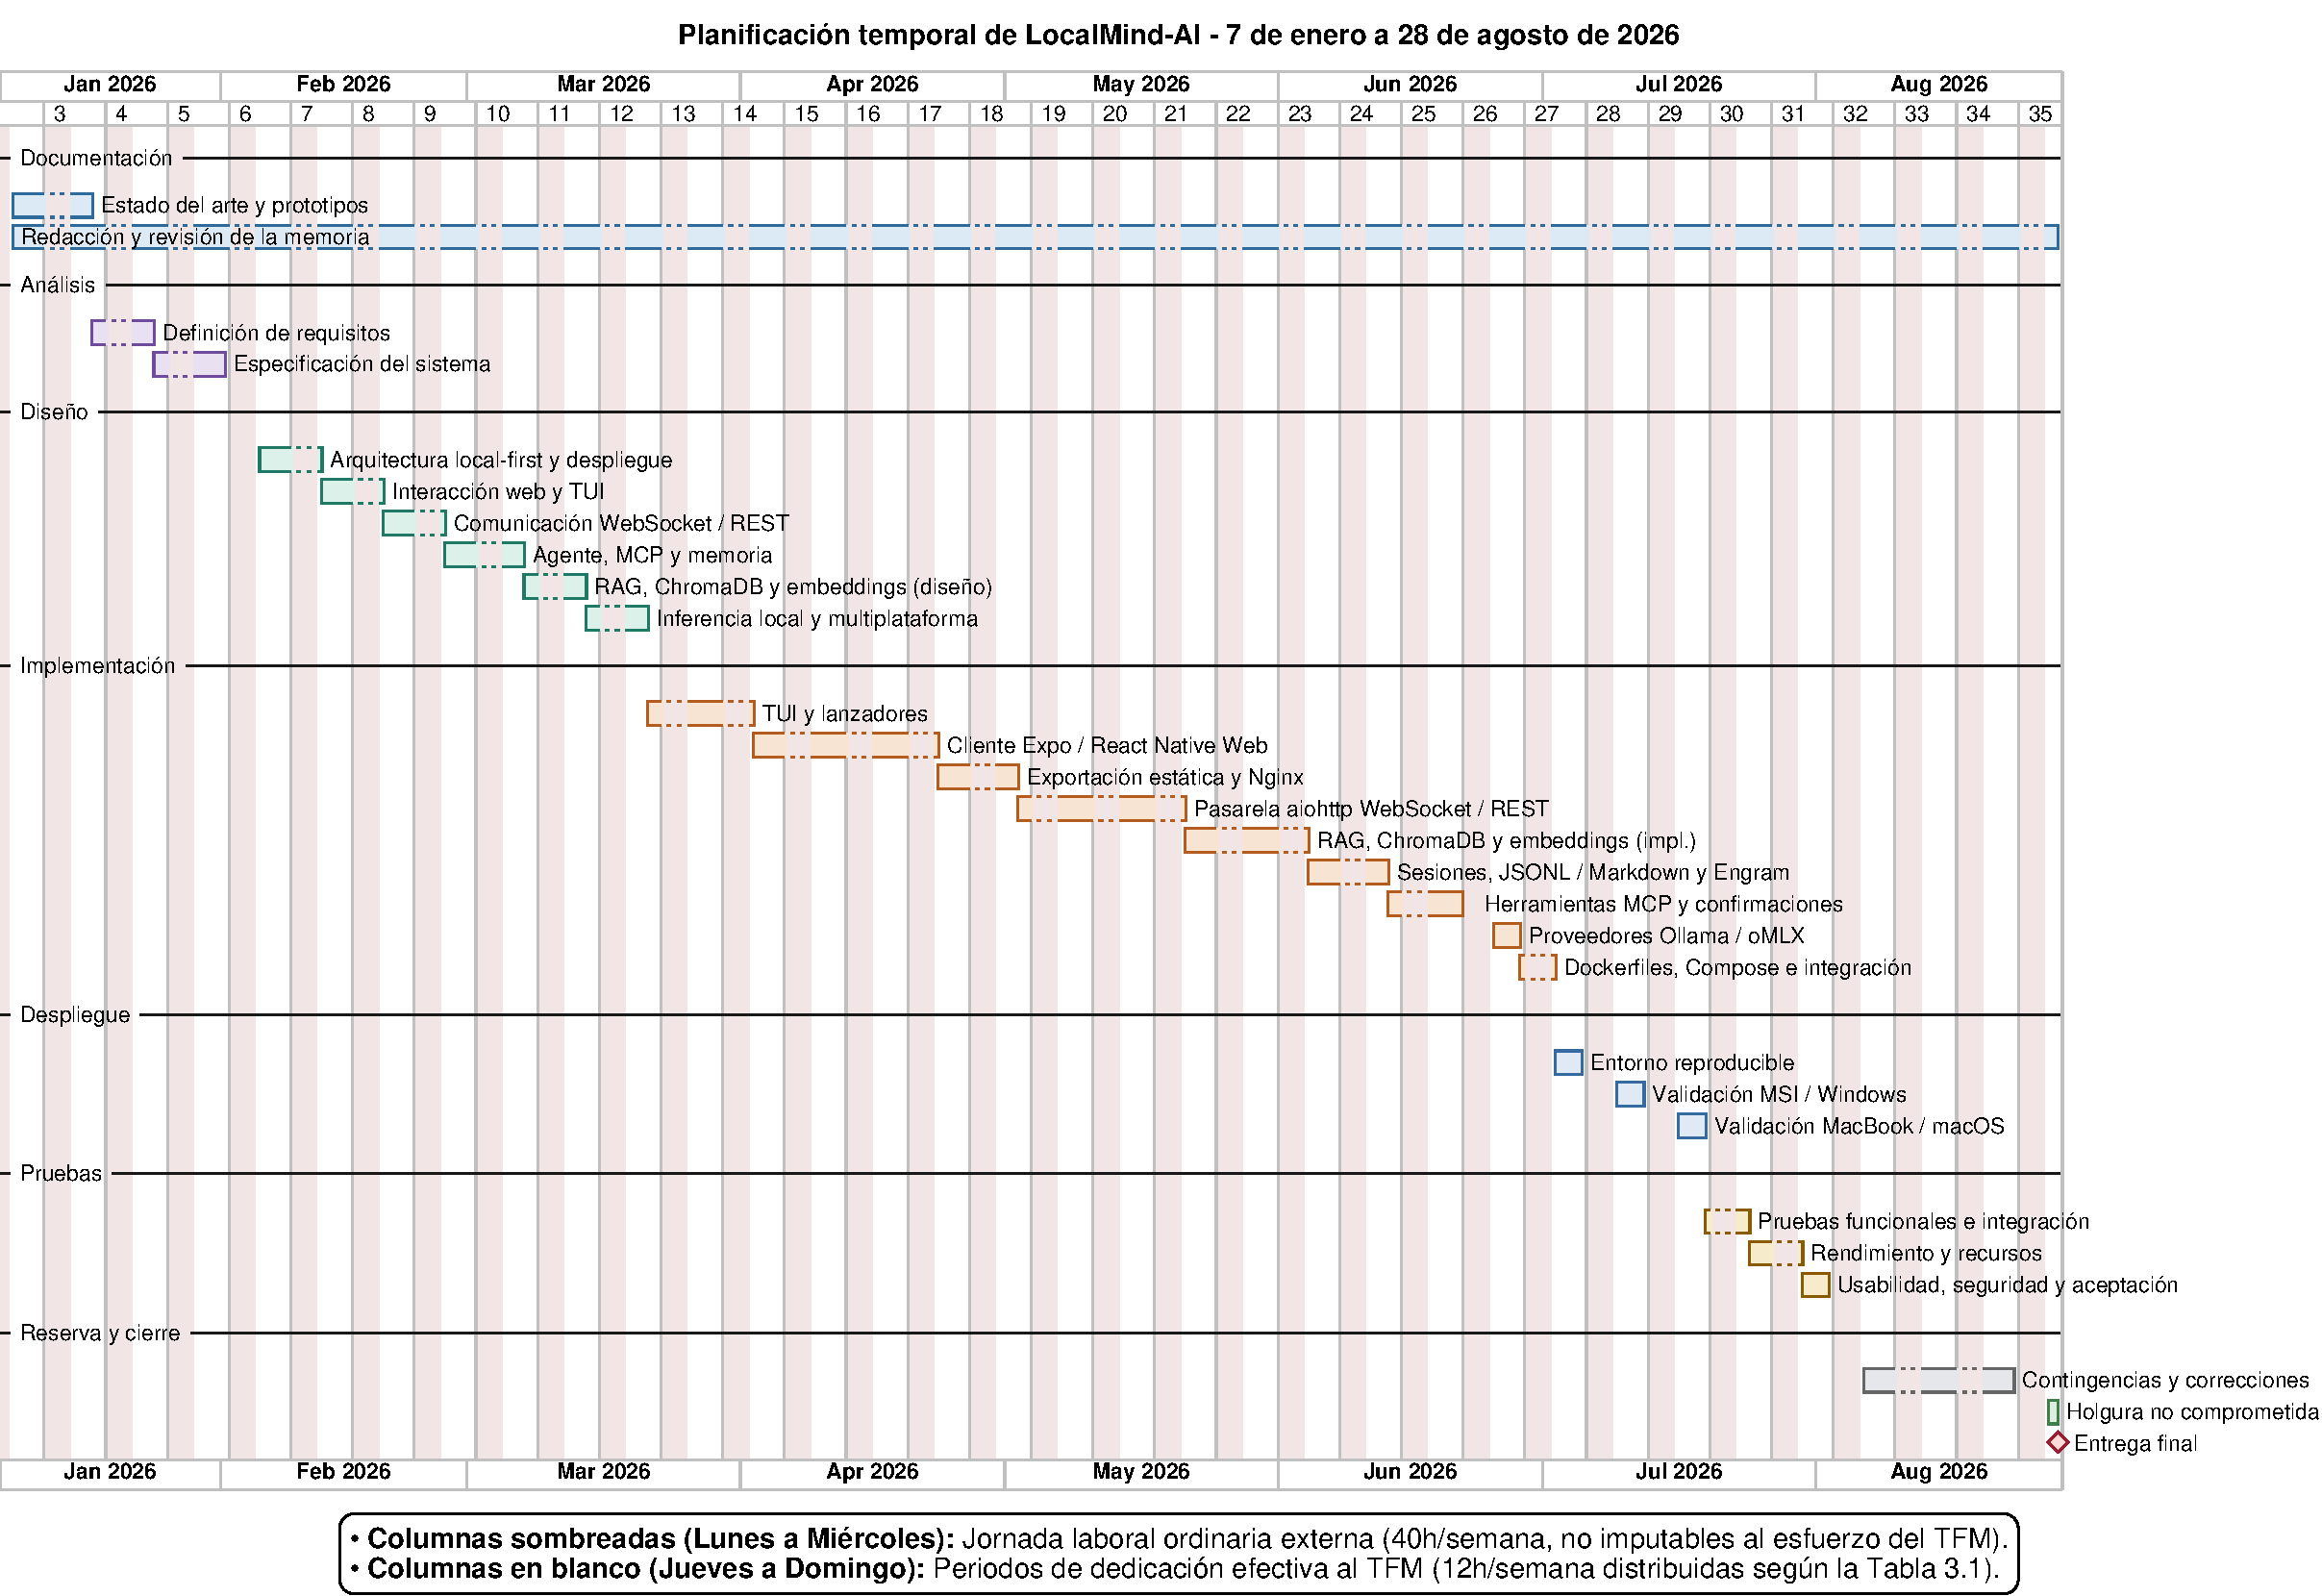
\includegraphics[width=0.98\textheight]{figs/GanttTFM.pdf}
    \caption{Diagrama de Gantt del proyecto, del 7 de enero al 28 de agosto de 2026.}
    \label{fig:diagramaGantt}
\end{sidewaysfigure}

\FloatBarrier

A efectos de estimación económica, el trabajo del autor se valora como el de un perfil \gls{fullstack} júnior. Glassdoor sitúa el salario medio del puesto en España en 22.744~\texteuro{} anuales y publica una equivalencia aproximada de 11~\texteuro{}/hora \cite{SueldoJuniorFull}. Esta tarifa se aplica a las 396 horas presupuestadas, por lo que el salario imputable asciende a 4.356,00~\texteuro{}. Para aproximar el coste empresarial se añade un 33\,\% en concepto de cotizaciones sociales \cite{SeguridadSocialCotizacion}; este porcentaje se utiliza como hipótesis presupuestaria y no como una liquidación laboral individual. El coste total del recurso humano resulta así de 5.793,48~\texteuro{}.

Las herramientas de desarrollo, bibliotecas y servicios utilizados se encuentran disponibles mediante licencias de código abierto, modalidades gratuitas o acceso académico ya disponible. Por ello, se asigna un coste directo de 0,00~\texteuro{} al \gls{software}. La electricidad, la conexión a Internet y los consumibles menores se consideran dentro de los costes indirectos.

Para valorar los equipos se emplea su precio de mercado consultado el 23 de julio de 2026. El MSI Pulse GL66 12UEK-085ES se valora en 917,80~\texteuro{} como equipo reacondicionado \cite{MSIPulseGL66}, mientras que el MacBook Air M4 de 13 pulgadas, con 16~GB de memoria unificada y 512~GB de almacenamiento, se valora en 1.109,00~\texteuro{} \cite{KtuinMacBookAirM4}. El HP OMEN utilizado como referencia descartada en el estado del arte no interviene en la ejecución ni se incorpora al presupuesto.

La tabla simplificada de la \gls{aeat} establece para los equipos informáticos un coeficiente máximo de amortización del 26\,\% y un periodo máximo de diez años \cite{AgenciaTributaria354}. Se adopta una vida útil de cuatro años y se imputa únicamente la fracción correspondiente a los 234 días naturales del proyecto. La Ecuación~\ref{eq:costematerial} formaliza este cálculo.

% Ecuación amortización del material.
\begin{equation}
    A_i = \frac{C_i}{4} \times \frac{234}{365}
    \label{eq:costematerial}
\end{equation}

En la ecuación, \(C_i\) representa el valor de mercado del equipo y \(A_i\) su coste amortizado. Cada amortización se redondea a céntimos antes de calcular los subtotales. La Tabla~\ref{tab:coste_amortizacion} muestra el resultado.

% Tabla de amortización de dispositivos.
\begin{table}[h!tp]
    \centering
    \begin{tabularx}{\textwidth}{|>{\raggedright\arraybackslash}X|>{\centering\arraybackslash}p{2.5cm}|>{\centering\arraybackslash}p{2.3cm}|>{\centering\arraybackslash}p{2.5cm}|}
        \hline
        \textbf{Equipo}                          & \textbf{Valor de mercado} & \textbf{Periodo imputado} & \textbf{Amortización} \\ \hline
        MSI Pulse GL66 12UEK-085ES               & 917,80~\texteuro{}        & 234 días                  & 147,10~\texteuro{}    \\ \hline
        MacBook Air M4 de 13 pulgadas, 16/512~GB & 1.109,00~\texteuro{}      & 234 días                  & 177,74~\texteuro{}    \\ \hline
    \end{tabularx}
    \caption{Valoración y amortización de los equipos utilizados.}
    \label{tab:coste_amortizacion}
\end{table}

Los costes directos se obtienen sumando el recurso humano, la amortización del hardware y el software. Sobre este subtotal se aplica un \textit{overhead} del 20\,\% para cubrir los costes indirectos. Como resume la Tabla~\ref{tab:costos}, el coste estimado del proyecto asciende a 7.341,98~\texteuro{}.

% Tabla de desglose de costes.
\begin{table}[h!tp]
    \centering
    \begin{tabular}{|>{\raggedright\arraybackslash}p{9cm}|>{\centering\arraybackslash}p{3.5cm}|}
        \hline
        \textbf{Concepto}                 & \textbf{Coste}                \\ \hline
        Recursos humanos                  & 5.793,48~\texteuro{}          \\ \hline
        Amortización del MSI Pulse GL66   & 147,10~\texteuro{}            \\ \hline
        Amortización del MacBook Air M4   & 177,74~\texteuro{}            \\ \hline
        Software y servicios              & 0,00~\texteuro{}              \\ \hline
        \textbf{Total de costes directos} & \textbf{6.118,32~\texteuro{}} \\ \hline
        Costes indirectos (20\,\%)        & 1.223,66~\texteuro{}          \\ \hline
        \textbf{Coste total}              & \textbf{7.341,98~\texteuro{}} \\ \hline
    \end{tabular}
    \caption{Desglose de costes del proyecto.}
    \label{tab:costos}
\end{table}

\FloatBarrier

\section{Riesgos}
% Riesgos que pueden afectar al desarrollo del sistema.
El carácter unipersonal del proyecto, su compatibilización con una jornada laboral y la integración de componentes heterogéneos introducen riesgos que pueden alterar la planificación. La Tabla~\ref{tab:risk_analysis} recoge los principales riesgos identificados, su desviación temporal estimada y la respuesta prevista. El coste expresa una demora potencial si se materializa el riesgo, no una reserva que deba añadirse automáticamente a las 396 horas presupuestadas.

\begin{table}[p]
    \centering
    \footnotesize
    \renewcommand{\arraystretch}{1.15}
    \begin{tabularx}{\textwidth}{
            |>{\raggedright\arraybackslash}p{4.2cm}
            |>{\centering\arraybackslash}p{2.1cm}
            |>{\raggedright\arraybackslash}X|
        }
        \hline
        \textbf{Riesgo} & \textbf{Coste}                                                                                                                                                                          & \textbf{Solución} \\ \hline
        Desviación del alcance al compatibilizar el \gls{tfm} con la jornada laboral
                        & Hasta 2 semanas
                        & Mantener cerrado el alcance del producto mínimo viable, revisar semanalmente el trabajo restante y posponer prototipos futuros antes de ampliar el calendario.                                              \\ \hline
        Instalación inconsistente entre \gls{windows} y \gls{macos}
                        & 5 días
                        & Ejecutar instalaciones limpias en el MSI y el MacBook, conservar diagnósticos reproducibles y documentar las diferencias entre \gls{ollama} y \gls{omlx}.                                                   \\ \hline
        Fallos de integración entre el cliente, \gls{nanobot}, \gls{websocket}/\gls{rest}, \gls{mcp}, \gls{rag} y la memoria
                        & 5 días
                        & Definir pruebas de contrato para cada frontera, integrar de forma incremental y conservar registros que permitan aislar el componente responsable.                                                          \\ \hline
        Recursos insuficientes o rendimiento inadecuado de los modelos
                        & 5 días
                        & Medir memoria y latencia por equipo, reducir contexto o cuantización y disponer de modelos alternativos de menor tamaño compatibles con el motor activo.                                                    \\ \hline
        Exposición de datos, credenciales o servicios locales
                        & 4 días
                        & Enlazar los servicios a la interfaz de bucle local, mantener los secretos fuera del código y solicitar confirmación antes de ejecutar acciones protegidas o activar servicios externos.                     \\ \hline
        Pérdida o corrupción de sesiones, memoria o colección vectorial
                        & 3 días
                        & Verificar los volúmenes persistentes, realizar copias de seguridad de los almacenes y probar su restauración antes de las validaciones finales.                                                             \\ \hline
        Cambios incompatibles en dependencias, modelos, interfaces o licencias
                        & 4 días
                        & Fijar versiones e identificadores, revisar las notas de publicación y mantener una alternativa conocida para cada dependencia crítica.                                                                      \\ \hline
    \end{tabularx}
    \caption{Análisis de riesgos, costes temporales y medidas de contingencia.}
    \label{tab:risk_analysis}
\end{table}

Las desviaciones de la tabla representan escenarios alternativos y, por tanto, no deben sumarse entre sí como si todos fueran a producirse. Si coincidieran varios riesgos graves y se agotara el margen previsto, se reduciría primero el alcance no esencial para preservar los requisitos del prototipo académico y la fecha de entrega.

\FloatBarrier

\section{Viabilidad}
% Viabilidad del proyecto presentado.
La viabilidad económica del proyecto es favorable dentro de su alcance académico. El coste estimado de 7.341,98~\texteuro{} incluye la valoración del trabajo y la amortización de los dos equipos, aunque no exige adquirirlos expresamente porque ambos se reutilizan. El coste directo de software y servicios se mantiene en 0,00~\texteuro{}, al emplearse soluciones de código abierto, gratuitas o disponibles mediante acceso académico.

Desde el punto de vista temporal, las 396 horas presupuestadas caben dentro de las 400 horas que proporciona el calendario. Sin embargo, la diferencia de cuatro horas es reducida y hace necesario controlar el alcance y aplicar las medidas de contingencia en cuanto se detecte una desviación. La duración total, superior a siete meses, no responde a una carga de trabajo a tiempo completo, sino a la dedicación de doce horas semanales compatible con una jornada laboral ordinaria de ocho horas diarias.

La viabilidad organizativa se encuentra condicionada por el desarrollo unipersonal. Esta configuración reduce el coste y facilita mantener una visión coherente del sistema, pero impide paralelizar actividades críticas y limita la revisión cruzada de decisiones. Para compensarlo, el proyecto se divide en incrementos verificables y reserva periodos específicos para validación, contingencias y correcciones.

La solución es técnicamente viable porque se apoya en tecnologías compatibles con la arquitectura descrita: un cliente web estático servido por \gls{nginx}, un agente \gls{nanobot} contenerizado, comunicación directa mediante \gls{websocket} y \gls{rest}, y motores de inferencia nativos \gls{ollama} u \gls{omlx}. No obstante, la viabilidad completa depende todavía de demostrar la instalación multiplataforma, el consumo de recursos, la persistencia, la observabilidad y las medidas de seguridad definidas en los requisitos.

La viabilidad operativa exige disponer de \gls{docker}, de un motor de inferencia compatible y de memoria suficiente para el modelo seleccionado. Una vez instaladas las dependencias y descargados los modelos, las funciones locales previstas deberán poder utilizarse sin conexión. Las integraciones externas no son necesarias para el funcionamiento básico y deben permanecer deshabilitadas hasta que exista una activación consciente.

En consecuencia, LocalMind-AI se considera viable como prototipo académico y personal, siempre que se mantenga el alcance definido y se completen las validaciones pendientes. Esta conclusión no equivale a afirmar que todos los objetivos de rendimiento, seguridad o compatibilidad se encuentren ya demostrados.

\subsection{Viabilidad legal}

El tratamiento de información en LocalMind-AI debe respetar el \gls{rgpd}, establecido por el Reglamento (UE) 2016/679 \cite{ReglamentoUE20162016}, y la \gls{lopdgdd}, que complementa este marco en España \cite{BOEA201816673LeyOrganica}. El enfoque local reduce transferencias innecesarias, pero no garantiza por sí solo el cumplimiento: siguen siendo necesarias la minimización de datos, la protección de credenciales, el control de los almacenes persistentes y la posibilidad de eliminar la información.

Las pruebas y demostraciones del \gls{tfm} utilizarán exclusivamente datos públicos o sintéticos. Si se habilita una herramienta o un proveedor externo, la persona usuaria deberá conocer y autorizar la transmisión antes de que se produzca. Esta cautela afecta también a \gls{engram}: la implementación configurada almacena la memoria en una base de datos local, pero su documentación contempla llamadas a un proveedor para \glspl{embeddings} y consolidación, con Gemini como opción predeterminada \cite{engramSdk2026}. Por ello, no se considera completamente desconectado hasta que su configuración concreta haya sido verificada.

El marco europeo aplicable a la \gls{ia} se encuentra en el Reglamento (UE) 2024/1689, denominado \gls{aiact}, cuya aplicación general comienza el 2 de agosto de 2026, sin perjuicio de las fechas específicas previstas para determinadas disposiciones \cite{ReglamentoUE20241689}. El prototipo deberá facilitar la supervisión humana, diferenciar las respuestas generadas y solicitar confirmación para acciones protegidas. No obstante, esta memoria no asigna al sistema una categoría jurídica definitiva de riesgo, ya que dicha clasificación depende del contexto de uso y de una evaluación legal que excede el alcance técnico del trabajo.

LocalMind-AI se presenta al cierre del \gls{tfm} como un prototipo académico y personal, sin distribución pública ni explotación comercial. El directorio raíz del proyecto no declara todavía una licencia propia, por lo que no debe interpretarse la disponibilidad local del código como una autorización de redistribución. Antes de una publicación futura sería necesario elegir una licencia compatible, conservar los avisos de terceros y revisar las condiciones de los modelos y de los servicios empleados.

La Tabla~\ref{tab:licencias} resume las licencias principales. Cuando un producto combina código abierto con una distribución o un servicio sujeto a términos adicionales, ambas condiciones se distinguen expresamente.

% Tabla de licencias tecnológicas.
\begin{table}[p]
    \centering
    \scriptsize
    \renewcommand{\arraystretch}{1.15}
    \begin{tabularx}{\textwidth}{
            |>{\raggedright\arraybackslash}p{3.6cm}
            |>{\raggedright\arraybackslash}p{3.1cm}
            |>{\raggedright\arraybackslash}X|
        }
        \hline
        \textbf{Software o recurso} & \textbf{Licencia o condiciones}                                                                                                                                                                                                                                                                                              & \textbf{Observaciones} \\ \hline
        \Gls{nanobot}, \gls{mcp}, \gls{aiohttp} y \gls{python}
                                    & \gls{mit}, \gls{apache2.0} y \gls{psfl}
                                    & Nanobot y el SDK de MCP se distribuyen bajo MIT, aiohttp bajo Apache 2.0 y Python bajo PSFL \cite{nanobot2026,mcpPythonSdk2026,aiohttpLicense2026,pythonLicense2026}.                                                                                                                                                                                 \\ \hline
        React, \gls{reactnative}, \gls{expo}, \gls{nodejs} y \gls{pnpm}
                                    & \gls{mit}
                                    & Los componentes de este grupo declaran licencias MIT en sus repositorios oficiales \cite{react2026,meta2024reactnative,expo2024,nodejs2026,pnpm2026}.                                                                                                                                                                                                 \\ \hline
        Docker Engine/Compose, Docker Desktop y \gls{nginx}
                                    & \gls{apache2.0}, términos de suscripción y \gls{bsd2}
                                    & Engine y Compose son proyectos Apache 2.0, Docker Desktop está sujeto a términos propios y Nginx utiliza BSD-2-Clause \cite{dockerEngineLicense2026,dockerComposeLicense2026,dockerDesktopTerms2026,nginxLicense2026}.                                                                                                                                \\ \hline
        \Gls{ollama}, \gls{mlx} y \gls{omlx}
                                    & \gls{mit} y \gls{apache2.0}
                                    & Ollama y MLX declaran MIT, mientras que oMLX declara Apache 2.0 \cite{ollamaLicense2026,mlxLicense2026,omlx2026}.                                                                                                                                                                                                                                     \\ \hline
        \Gls{chromadb} y Engram SDK
                                    & \gls{apache2.0} y \gls{mit}
                                    & ChromaDB declara Apache 2.0 y el paquete \texttt{engram-sdk} MIT, el cual puede utilizar proveedores externos según su configuración \cite{chroma2026,engramSdk2026}.                                                                                                                                                                                 \\ \hline
        Ornith-1.0-9B (4-bit / 6-bit), Qwen3.5-9B-Instruct (4-bit / 6-bit), Qwopus3.5-9B-Coder (4-bit / 6-bit) y Qwopus3.5-4B-Coder (4-bit / 6-bit)
                                    & \gls{mit} y \gls{apache2.0}
                                    & Las versiones cuantizadas de Ornith-1.0-9B en 4 y 6 bits declaran MIT en HuggingFace, mientras que los modelos Qwen3.5-9B-Instruct y Qwopus3.5-Coder en sus variantes de 9B y 4B parámetros con cuantizaciones de 4 y 6 bits o esquemas Q4\_K\_M y Q6\_K se distribuyen bajo Apache 2.0 \cite{ornith9b4,ornith9b6,qwen359b}.                          \\ \hline
        \Gls{git} y GitHub
                                    & \gls{gpl2only} y términos de servicio
                                    & Git se distribuye bajo GPL-2.0-only, mientras que el alojamiento y las funciones de GitHub se rigen por sus condiciones de servicio \cite{gitLicense2026,githubTerms2026}.                                                                                                                                                                            \\ \hline
        \Gls{latex}, \gls{mactex} y \gls{plantuml}
                                    & \gls{lppl}, licencias múltiples y \gls{gnugpl3}
                                    & LaTeX utiliza LPPL, MacTeX agrupa componentes con licencias propias y PlantUML se distribuye bajo GPL v3 \cite{latexLicense2026,mactex2026,plantumlLicense2026}.                                                                                                                                                                                      \\ \hline
        Zotero, Visual Studio Code y Visual Paradigm
                                    & \gls{agpl3}, MIT o propietaria y propietaria académica
                                    & Zotero declara AGPL v3, Code-OSS es MIT, la distribución de Microsoft se rige por su licencia de producto y Visual Paradigm utiliza condiciones propietarias para su edición académica \cite{zoteroLicense2026,vscodeLicense2026,VisualParadigmLicensing}.                                                                                            \\ \hline
    \end{tabularx}
    \caption{Licencias y condiciones de las tecnologías empleadas.}
    \label{tab:licencias}
\end{table}

\FloatBarrier
